\section{Estado del arte}

La tecnología robótica se encuentra en plena fase de crecimiento, y por lo tanto, es previsible una presencia cada vez mayor de los robots, tanto en el sector industrial y de servicios, como en el sector doméstico. Como ha ocurrido en la informática, el desarrollo de robots se hace cada vez más accesible y por consiguiente sus capacidades tienden cada vez mayores gracias al aporte de una comunidad en auge. Este aumento en el interés de las personas sobre esta área, plantea ciertos desafíos, no solo en los aspectos tecnológicos, sino, también desde el punto de vista cultural y ético.

En la última mitad del siglo pasado el foco estaba puesto sobre todo en el campo de la robótica para impulsar el desarrollo de la producción a gran escala. Hoy se ha logrado gracias a ello un nivel tal de tecnología que el estudio y la realización de robots flexibles capaces de adaptarse a diferentes propósitos a diferentes entornos de trabajo ya no es una utopía. Desde el año dos mil, la investigación en el campo robótico también se dirige hacia el diseño de robots dedicados a la exploración del medio ambiente y de los llamados "robots de servicio".

Si hacemos foco en lo que respecta a los robots exploradores móviles, los mayores avances tecnológicos se dan en la exploración de otros planetas. Actualmente los científicos están enfocados en el planeta Marte así como lo fue en su momento la superficie Lunar. Los primeros desarrollos de este tipo de vehículos no tripulados surgen principalmente durante la carrera espacial entre USA y la URSS en la década del 60/70, donde los más conocidos, exceptuando los exploradores lunares han sido los siguientes:

Mars3 enviado en 1971 por la URSS el cual funcionó sobre la superficie marciana durante unos escasos 20 segundos.

\begin{figure}[H]
    \centering
    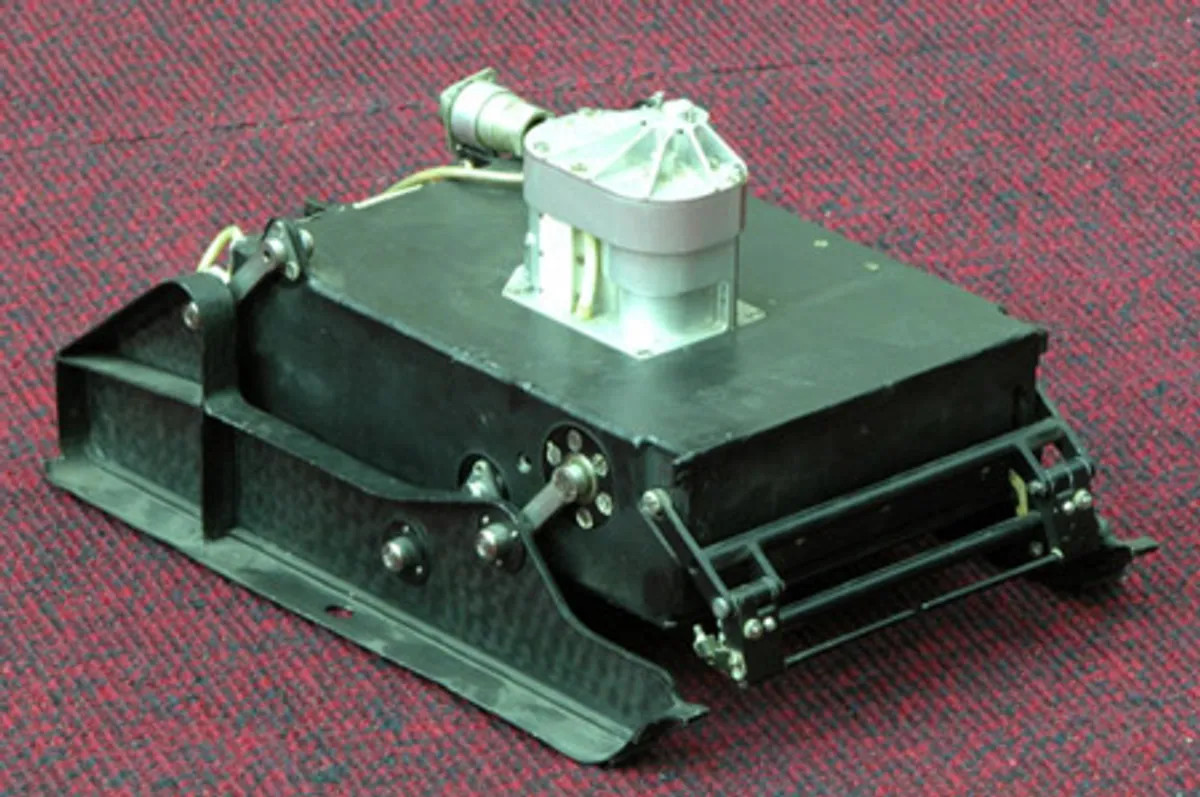
\includegraphics[width=0.5\linewidth]{images/mars3.jpg}
    \caption{Robot Mars3}
    \label{fig:mars3}
\end{figure}

En 2003, la NASA envió dos vehículos idénticos de 174 kilogramos con seis ruedas y paneles solares para recorrer parte de la superficie marciana, el Spirit y el Opportunity. El primero transmitió datos que hacen pensar que en el pasado existió agua líquida en Marte, hasta que se atasco y dejó de funcionar. El Opportunity todavía está operativo y ostenta el récord de distancia recorrida en otro planeta, con más de 42,6 kilómetros hasta el momento.

\begin{figure}[H]
    \centering
    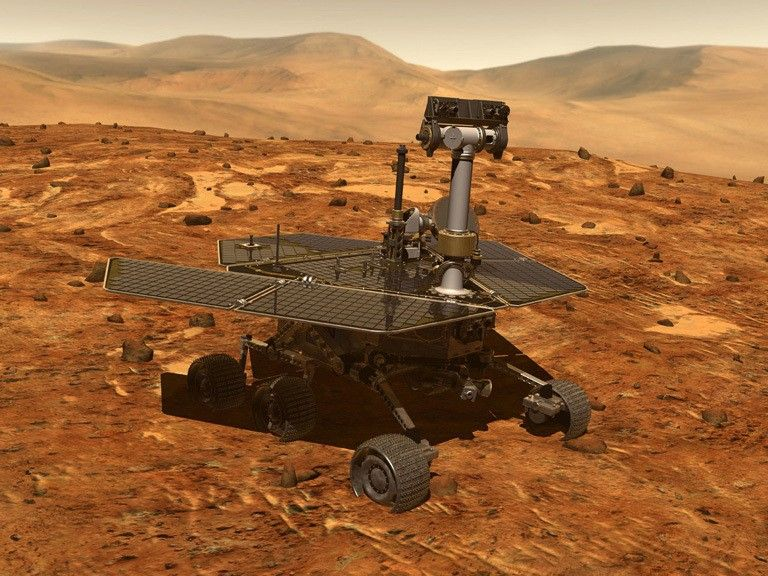
\includegraphics[width=0.5\linewidth]{images/opportunity-3d-model.jpg}
    \caption{Robot Opportunity}
    \label{fig:robot_opportunity}
\end{figure}

En 2011 la NASA envió a Marte el Curiosity, el Rover más grande y pesado lanzado hasta ese momento, aún se encuentra operativo y ha aportado las primeras evidencias de moléculas orgánicas en el planeta rojo.

\begin{figure}[H]
    \centering
    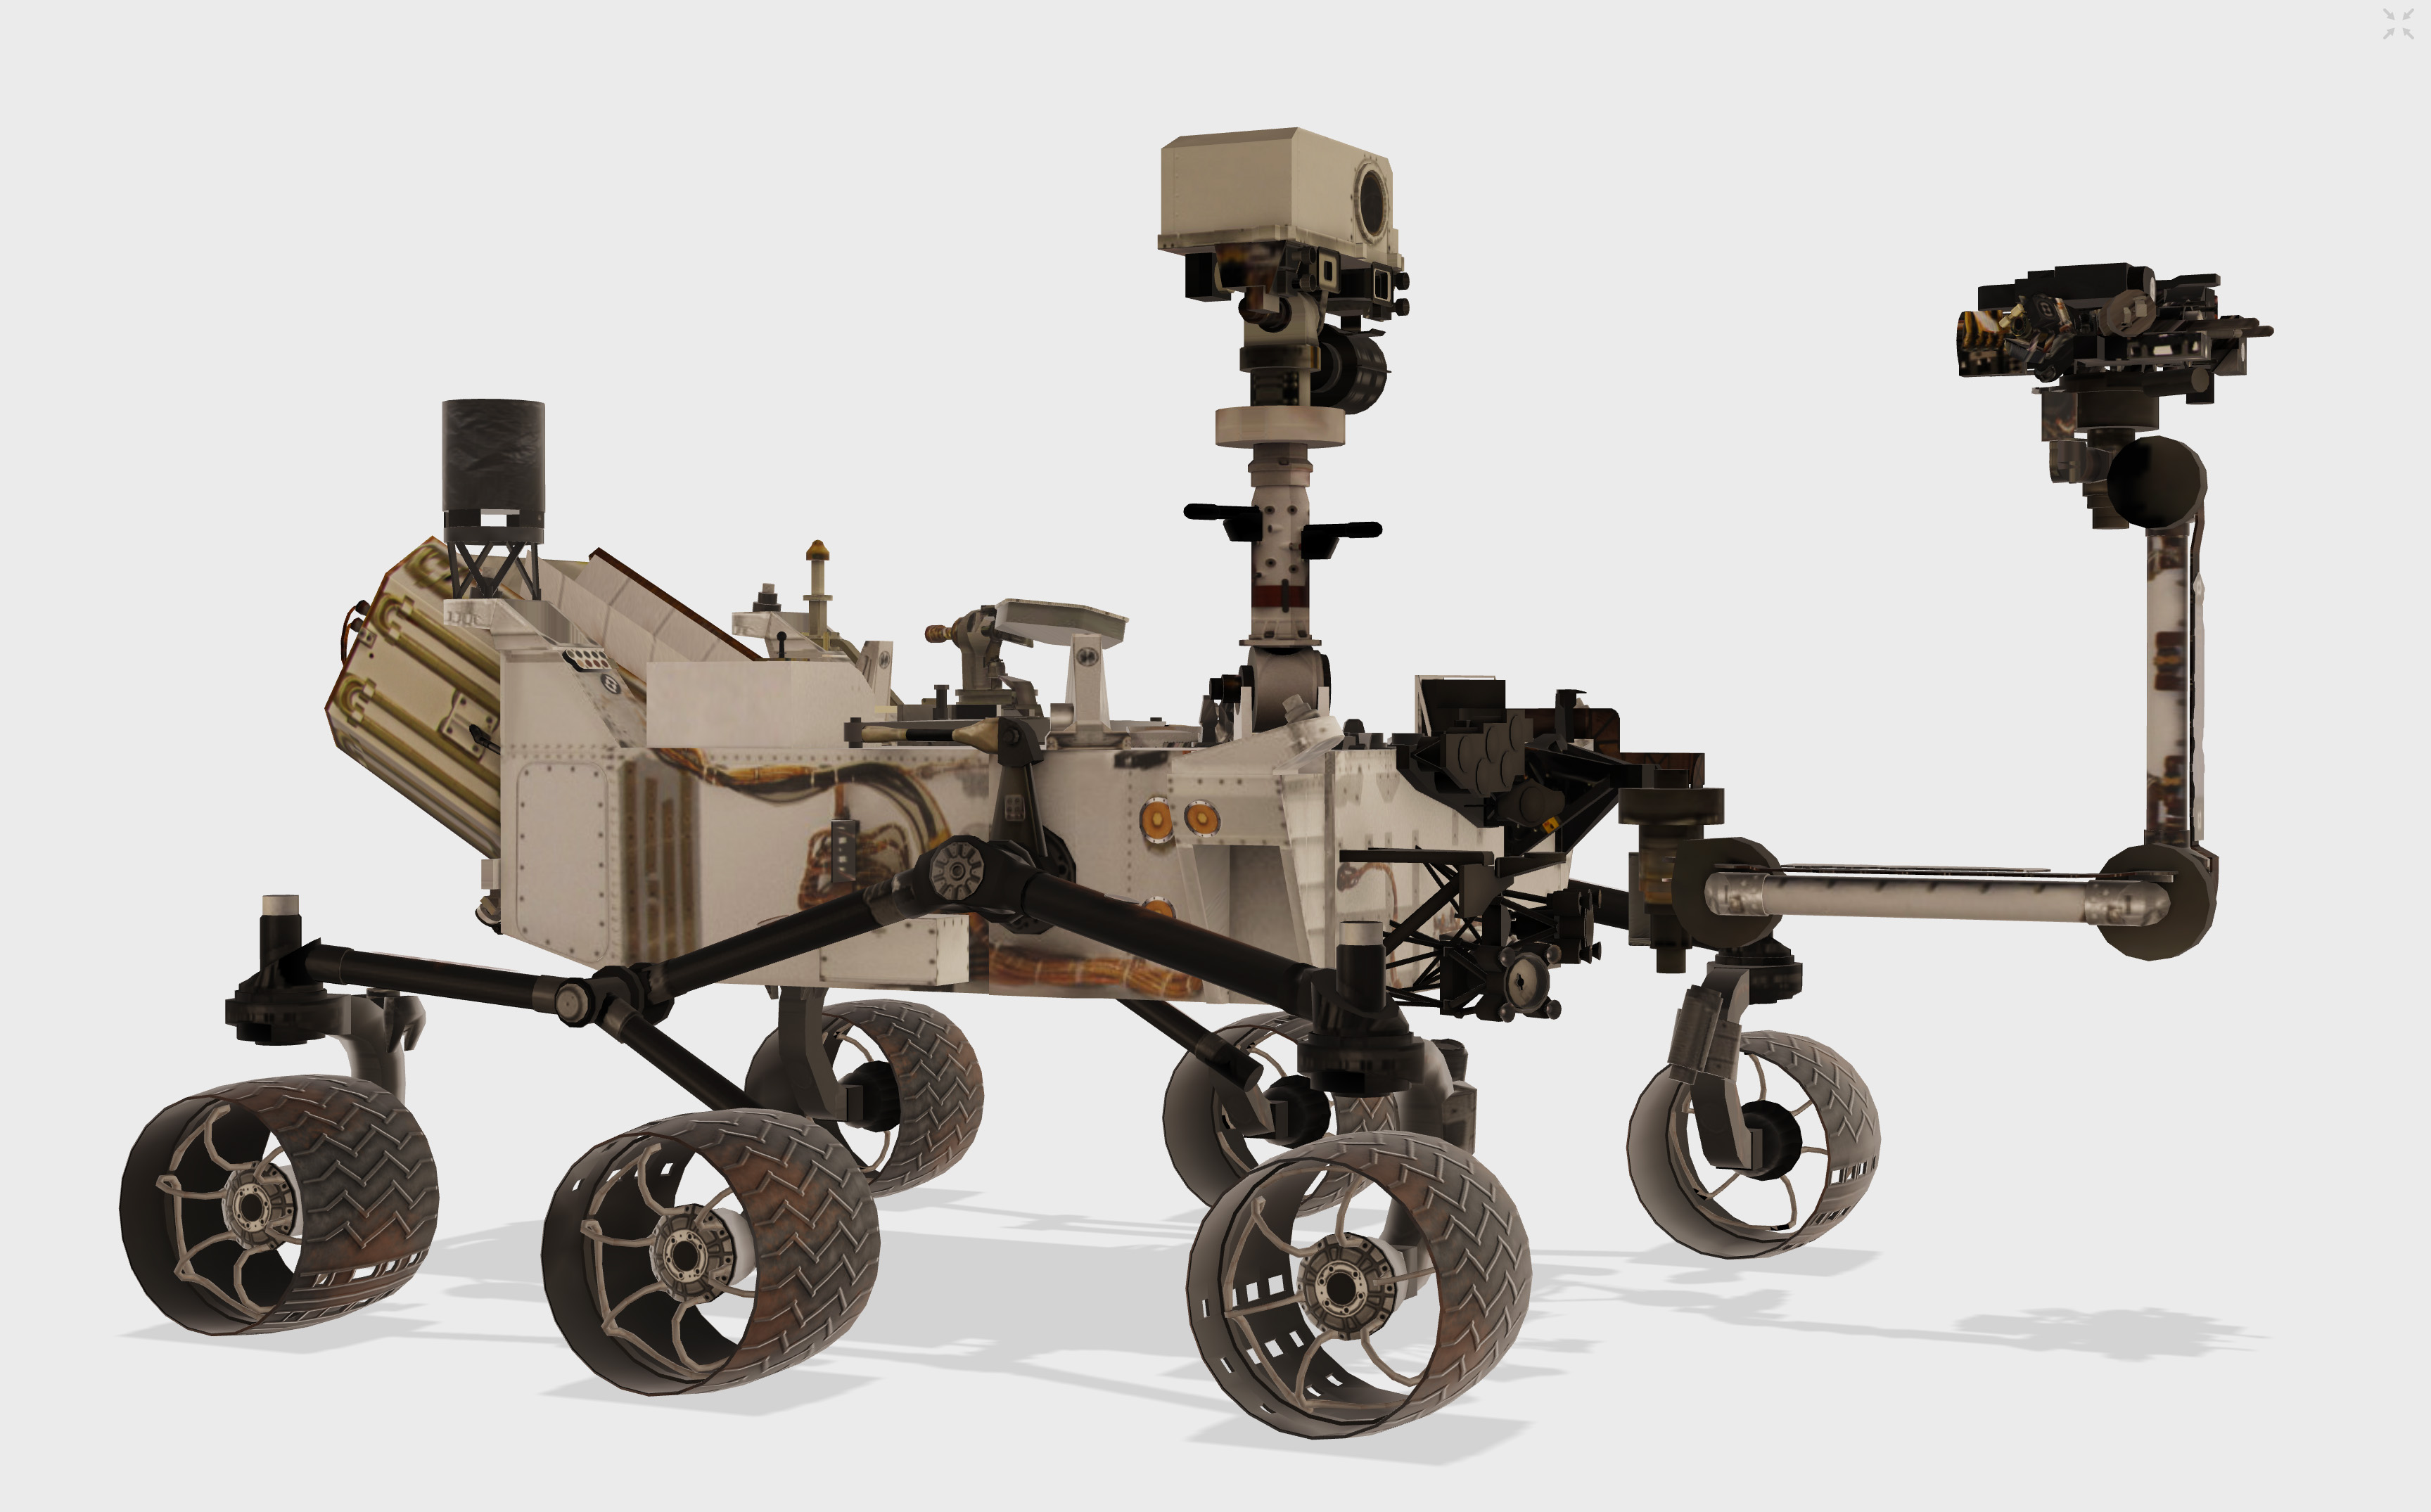
\includegraphics[width=0.5\linewidth]{images/curiosity-3d-model.jpg}
    \caption{Robot Curiosity}
    \label{fig:robot_curiosity}
\end{figure}

El 14 de marzo de 2016 la ESA y la Roscosmos enviaron a Marte la misión ExoMars, la primera de dos misiones que buscan analizar la atmósfera y colocar en su superficie dos vehículos, el segundo (2018) capaz de excavar dos metros por debajo de la superficie.

\begin{figure}[H]
    \centering
    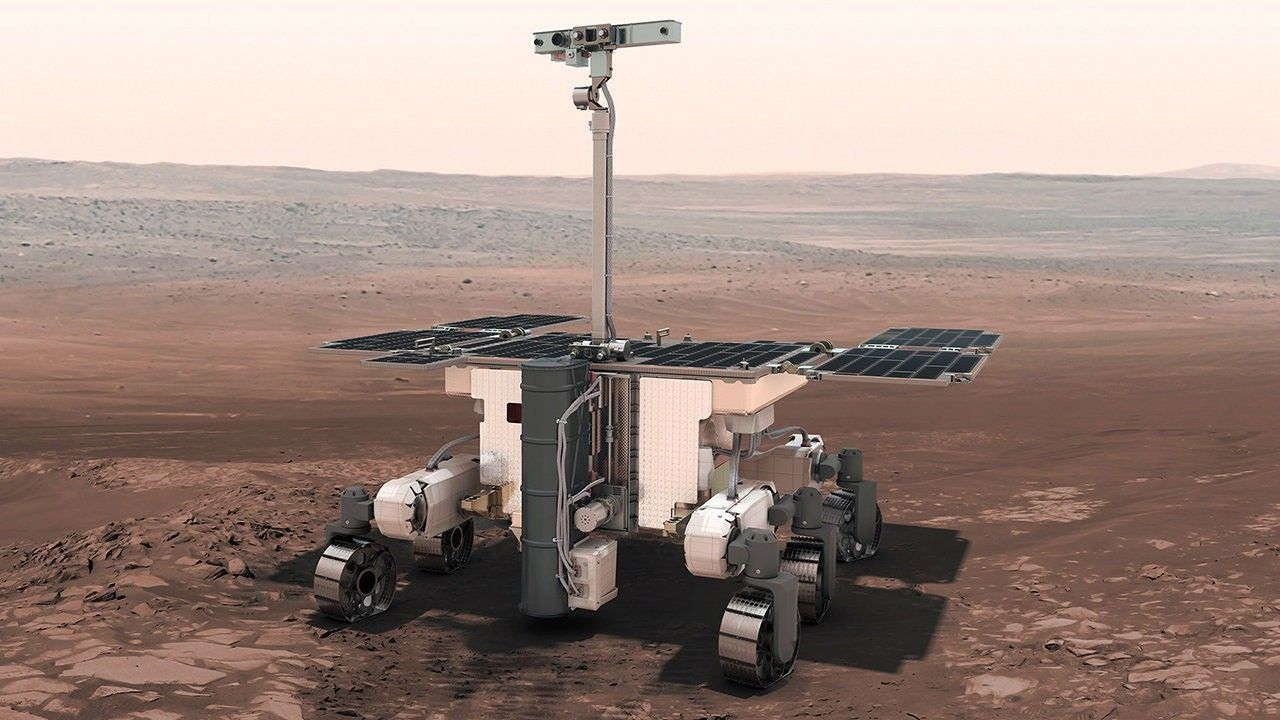
\includegraphics[width=0.5\linewidth]{images/Exomars_Rover.jpg}
    \caption{Robot ExoMars Rover}
    \label{fig:robot_exomarsrover}
\end{figure}

Por otra parte, tenemos a la robótica de servicio que es útil en el campo de la robótica médica, para la asistencia en rehabilitación y cirugía, así como en el campo doméstico para realizar tareas de limpieza y vigilancia.

La robótica móvil para estos sectores se ha convertido en una "herramienta de trabajo" importante y cada vez adquiere mayor protagonismo.

En los últimos años, mientras que la investigación de punta se enfoca en el diseño de robots para la exploración de Marte, en virtud de las tecnologías desarrolladas para tal fin, se hicieron los primeros robots para uso civil. Algunos de ellos, gracias a su pequeño tamaño y bajo costo de producción, gozan de cierto éxito comercial. Podemos mencionar de ejemplos al robot Roomba, hecho para la limpieza y lavado de pisos, una tarea que podría considerarse sencilla pero que implica un intenso trabajo computacional.

Sea cual sea el ámbito de aplicación, el diseño de robots móviles de pequeño tamaño y bajo costo de producción, pero, equipados con lógica de control avanzada, ha demostrado ser una gran utilidad para el hombre.